\titleformat{\chapter}[display]{\bfseries\centering}{\huge Chapter \thechapter}{1em}{\Huge #1}
\newgeometry{top=3cm, bottom=2.2cm, left=3cm, right=2cm, headsep=1.2cm, footskip=1cm, headheight=0.3cm, textheight=24.5cm, textwidth=16cm}
\onehalfspacing
\pagestyle{fancy}
\fancyhf{}
\renewcommand{\headrulewidth}{0pt}
\lhead{Chapter 3}
\rhead{Proposed System}
\cfoot{\thepage}
\chapter{Proposed System}

\section{Detailed Explanation of the Proposed System}
\noindent Sentinel is built in five layers (Figure~\ref{fig:arch}):
\begin{enumerate}
\item \textbf{Input:} the web app and the Chrome extension collect a message, link, chat, profile or account, or read the visible text of a page when auto-scan is on.
\item \textbf{Preprocessing:} the server checks that the request is valid and safe. Links are read as text only and never opened.
\item \textbf{Threat detection:} separate checkers look at the input: fraud rules, harm rules, the scam-text model, the community matcher, profile checks and bot detection.
\item \textbf{Analysis:} each checker gives its own level (for example High, Review or Low concern) with its evidence. Results are never merged into one score.
\item \textbf{Output:} the results appear as cards in the web app, in the extension popup, or as markers on the web page. The user can save a case.
\end{enumerate}

\noindent\textbf{Working principle.} Every result says what was \emph{observed}, what \emph{could not be checked}, and what to do next, so ``nothing found'' is never shown as ``safe''. A learned model is used only if its files pass a checksum test and the model passed its release test; if it fails at run time, its card says ``unavailable'' and the rules still work.

\begin{figure}[H]
\centering
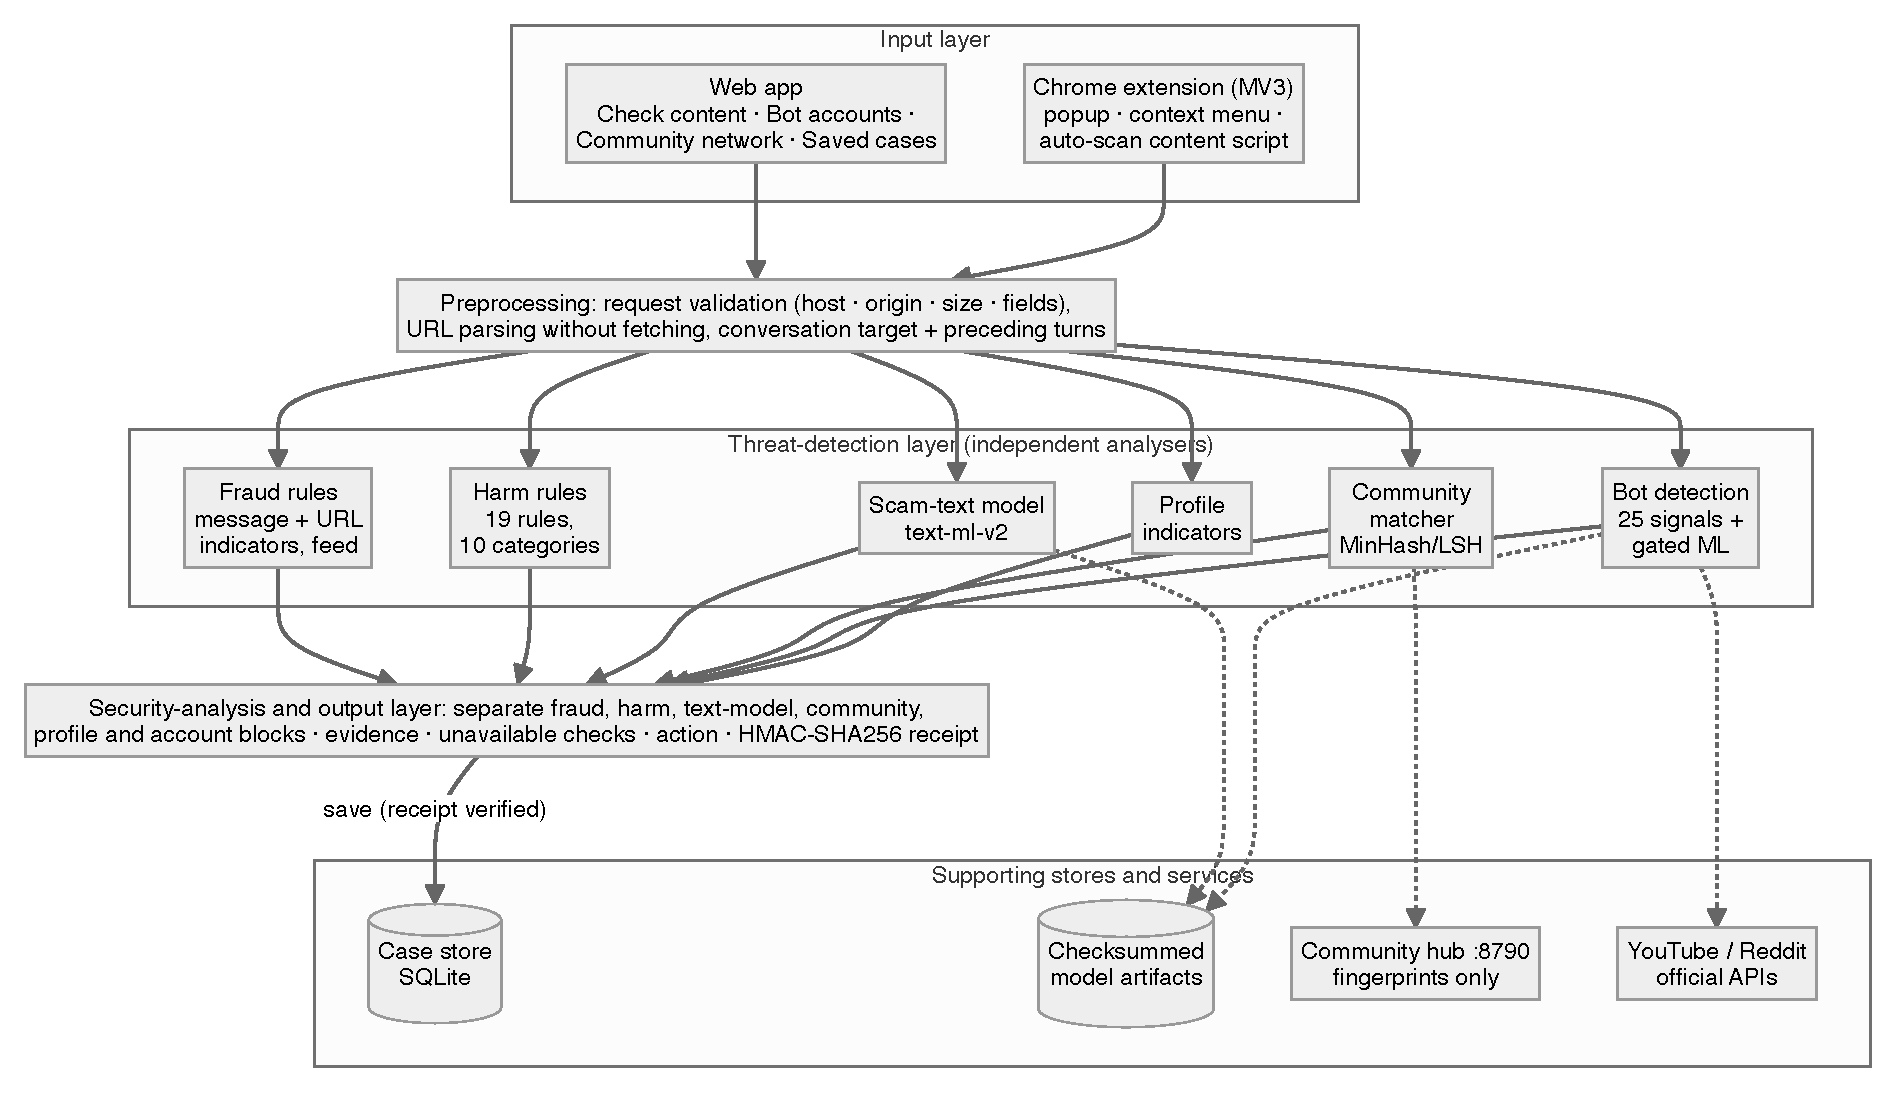
\includegraphics[width=0.95\linewidth]{dia2/arch_v2.pdf}
\caption{Layered architecture of Sentinel}
\label{fig:arch}
\end{figure}

\subsection{Module-wise Explanation}
\begin{enumerate}[label=\textbf{M\arabic*}, leftmargin=1.1cm]
\item \textbf{Web app:} four pages: \emph{Check content}, \emph{Bot accounts}, \emph{Community network} and \emph{Saved cases}. Results are shown as cards; a high-risk harm card moves to the top.
\item \textbf{Chrome extension:} a popup and right-click menu for quick checks, plus \emph{auto-scan}. When the user turns auto-scan on for a site, the extension reads the text visible on screen, sends it in small batches to the local server and marks risky messages without changing the page. It can also read text and QR codes inside images on that site, using OCR that runs inside the extension. If the server is off, it waits and retries; it never shows anything as ``safe''.
\item \textbf{Local server (\texttt{server.py}):} a Python web server that only listens on the user's own computer. It rejects requests from other websites, limits request size and adds browser security headers.
\item \textbf{Fraud rules:} look for requests for money or fees, passwords or OTPs, and urgency, and for suspicious links (an IP address instead of a name, ``@'' in the address, punycode, very long links). An optional list of known phishing links can be loaded.
\item \textbf{Harm rules:} 19 rules in 10 groups, such as threats, self-harm, sextortion, blackmail, stalking, hate and harassment, in English and Hinglish. They first undo disguises (\texttt{1d10t}$\to$idiot, \texttt{k.y.s}$\to$kys) and then check context: idioms (``this movie killed it'') are ignored, ``I would never hurt you'' is not a threat, and quoted insults go to human review. Self-harm messages get helpline numbers (Tele-MANAS 14416) \cite{telemanas}.
\item \textbf{Scam-text model (text-ml-v2):} a DistilBERT model and a TF-IDF model, averaged. It labels a message as genuine, spam or smishing, gives a probability, and highlights the words that raised the score.
\item \textbf{Batch scan:} the auto-scan endpoint. It runs all checks on up to 40 page items at once and gives each a severity: high, review or none.
\item \textbf{Community network:} when a user's Sentinel finds a scam, it can (if the user agrees) send only a \emph{fingerprint} of it to a hub. When 5 different users report the same scam, the hub publishes it, and every user is warned, even if their own model missed it. The hub never sees the message text.
\item \textbf{Bot detection:} takes a profile link, an uploaded file or typed details, and gets data only from the official YouTube or Reddit APIs or from the user. It scores 25 signals (posting rhythm, repeated posts, follower ratio and others) and shows which signals mattered. A trained activity model adds a probability for X accounts.
\item \textbf{Profile checks:} simple flags such as very many posts per day or following far more accounts than follow back.
\item \textbf{Receipts and case store:} each result carries a signed receipt (HMAC). A case can be saved only with a valid receipt, so the saved result is exactly what the user saw. Cases are stored in a local SQLite file and can be exported or deleted.
\item \textbf{Research pipeline:} command-line tools to download datasets (checked by SHA-256), split them fairly, train, calibrate and test models once on held-out data.
\end{enumerate}

\section{System Analysis}
\subsection{Functional Requirements}
\begin{enumerate}[label=FR\arabic*:, leftmargin=1.3cm]
\item Accept a message, link, chat, profile details or account, alone or together.
\item Reject empty, too large or invalid requests with a clear error.
\item Report fraud, harm, model, community and account results separately, each with evidence, missing checks and an action.
\item Never open a submitted link or scrape a profile.
\item Detect harmful language in English and Hinglish and give advice by urgency.
\item Scan visible page text only on sites the user switched on, and mark risky items.
\item Share only anonymous fingerprints with the hub, and only if the user agrees.
\item Analyse accounts from official APIs, uploads or manual entry; reject unsafe profile links.
\item Save, list, export and delete cases; save only with a valid receipt.
\end{enumerate}

\subsection{Non-Functional Requirements}
\begin{itemize}
\item \textbf{Privacy:} everything runs on the user's computer; nothing is stored unless saved; the hub stores no message text.
\item \textbf{Security:} local-only server, origin checks, size limits, security headers, signed receipts, safe link parsing, rate limits, API keys only from environment variables.
\item \textbf{Explainability:} every result explains its evidence in plain words.
\item \textbf{Performance:} rule checks take milliseconds; the text model takes about 2 ms per message on a laptop CPU.
\item \textbf{Reliability:} a broken model or offline hub shows ``unavailable''; it never breaks the check.
\item \textbf{Portability:} runs on Windows, macOS or Linux with Python and Chrome.
\end{itemize}

\subsection{Software and Hardware Requirements}
\begin{table}[H]
\centering
\small
\renewcommand{\arraystretch}{1.2}
\caption{Software and hardware requirements}
\label{tab:swhw}
\begin{tabular}{|>{\raggedright\arraybackslash}p{3.5cm}|>{\raggedright\arraybackslash}p{11.3cm}|}
\hline
\textbf{Component} & \textbf{Requirement} \\ \hline
Operating system & Windows 10/11, macOS or Linux \\ \hline
Application & Python 3.10+ (rules need only the standard library); SQLite \\ \hline
Models & ONNX Runtime, \texttt{tokenizers}, scikit-learn, NumPy; PyTorch and Transformers only for training \\ \hline
Browser and tests & Google Chrome; Python \texttt{unittest}; Node.js for JavaScript tests \\ \hline
Hardware & Laptop with 16 GiB RAM (AMD Ryzen 7 7435HS or Apple M4) \\ \hline
Network & Not needed for checks; only for the optional YouTube/Reddit APIs and dataset downloads \\ \hline
\end{tabular}
\end{table}

\subsection{Use Case Modelling}
\noindent Figure~\ref{fig:usecase} shows the main actors: the \emph{User}, the \emph{Research team member} and the optional \emph{Phishing feed}. Table~\ref{tab:uc} summarises the main use cases, including those added in this phase.
\begin{figure}[H]
\centering
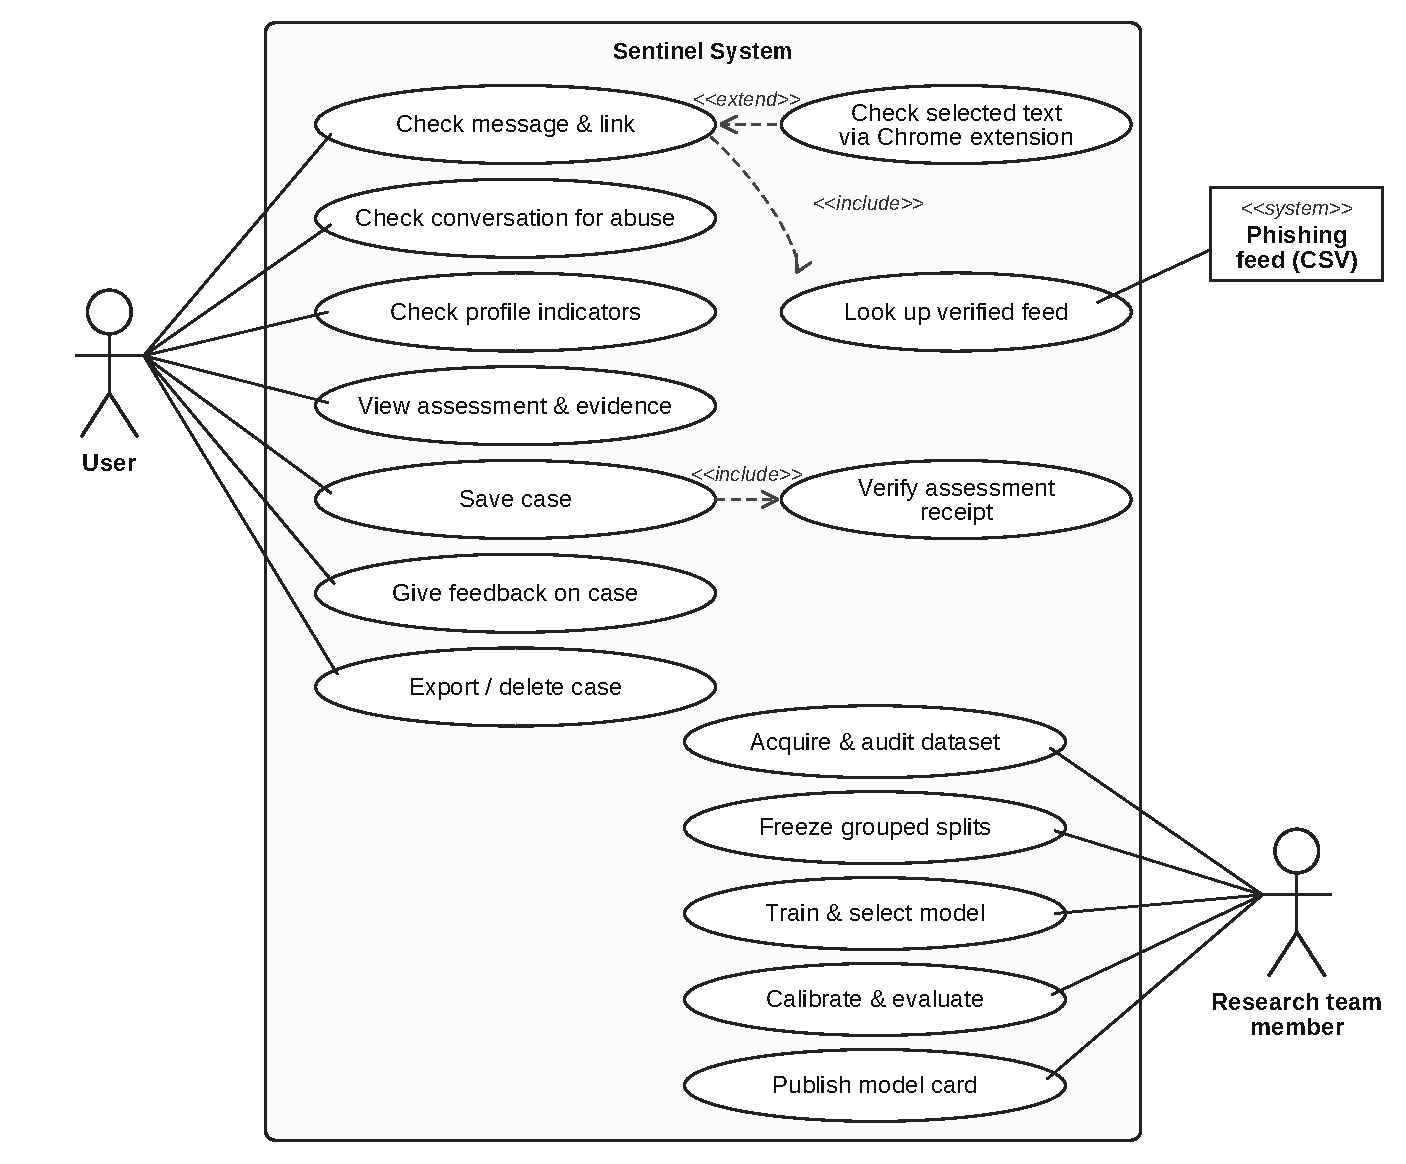
\includegraphics[width=0.82\linewidth]{dia/usecase.pdf}
\caption{Use case diagram (core check)}
\label{fig:usecase}
\end{figure}

\begin{table}[H]
\centering
\footnotesize
\renewcommand{\arraystretch}{1.2}
\caption{Main use cases}
\label{tab:uc}
\begin{tabular}{|l|>{\raggedright\arraybackslash}p{2.6cm}|>{\raggedright\arraybackslash}p{7.2cm}|>{\raggedright\arraybackslash}p{3.3cm}|}
\hline
\textbf{ID} & \textbf{Use case} & \textbf{Main steps} & \textbf{Result} \\ \hline
UC-01 & Check a message and link & Paste content, click \emph{Analyze}; server validates and runs all checkers; result cards appear & Cards with evidence; nothing stored \\ \hline
UC-02 & Save a case & Click \emph{Save}; server checks the receipt (same input, under 15 min) and stores the case & Case listed; can export or delete \\ \hline
UC-03 & Auto-scan a page & Turn auto-scan on for a site; visible text is batched and scanned; risky items are marked & Markers and badge count; page unchanged \\ \hline
UC-04 & Check an account & Enter a link or upload posts; data comes from an official API or the file; 25 signals are scored & Score, confidence and top signals \\ \hline
UC-05 & Train and test a model & Download and verify data, split, train, calibrate, test once & Model card; released only if it passes \\ \hline
\end{tabular}
\end{table}

\section{Proposed System: Analysis, Modelling and Design}
\noindent The activity, sequence, class, ER and data-flow diagrams below describe the core content check; a second sequence diagram shows auto-scan, and the deployment diagram shows all parts.

\subsection{Activity Diagram}
\noindent Figure~\ref{fig:activity} follows one check: the request is checked, the checkers run side by side, and the result is shown and optionally saved.
\begin{figure}[H]
\centering
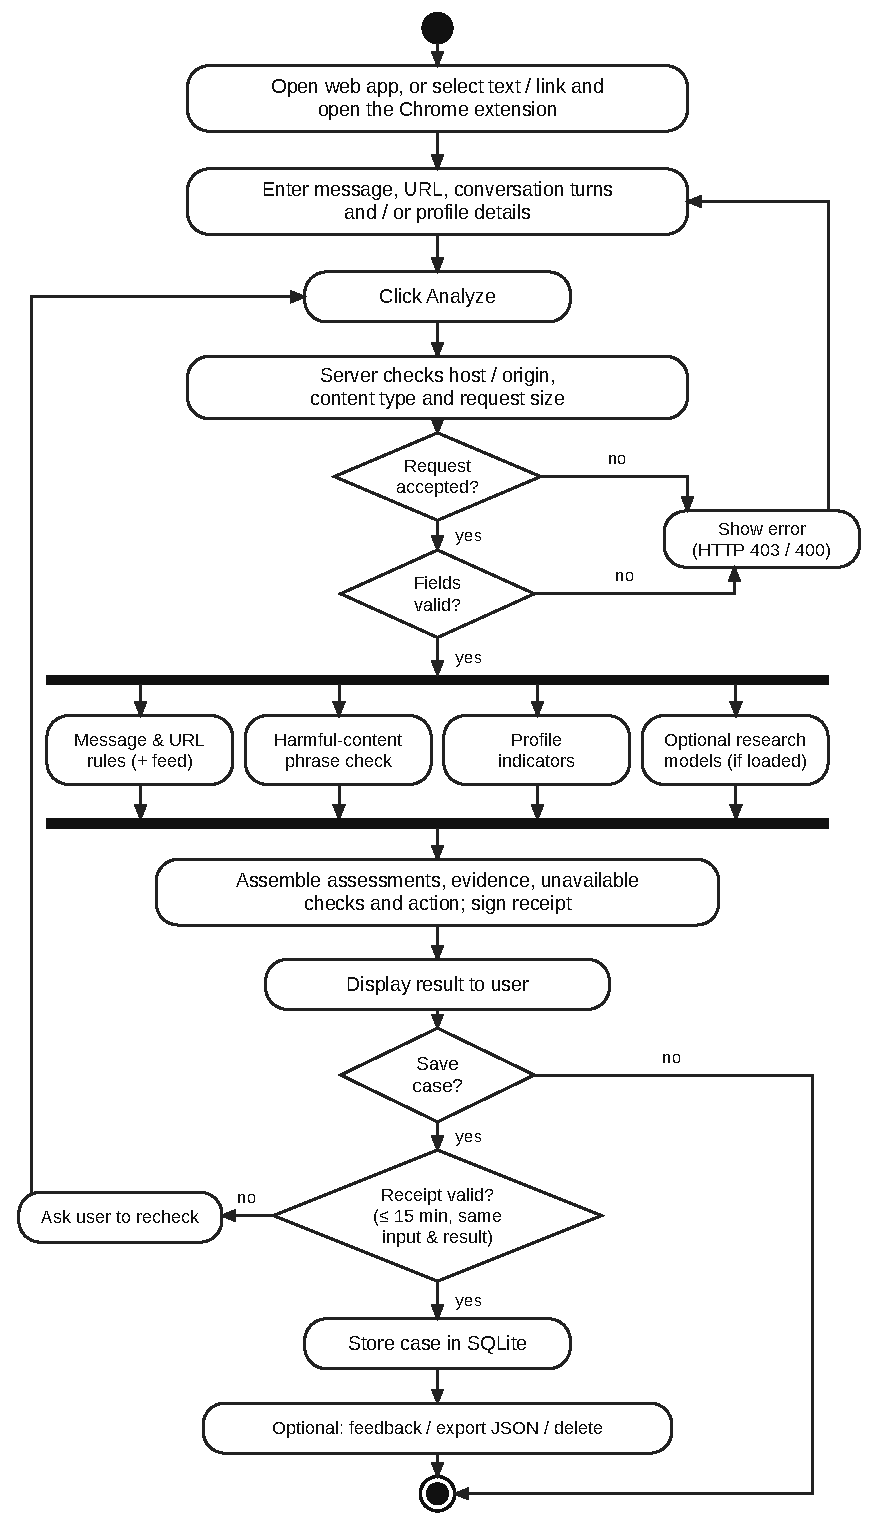
\includegraphics[height=0.62\textheight]{dia/activity.pdf}
\caption{Activity diagram of a Sentinel check}
\label{fig:activity}
\end{figure}

\subsection{Sequence Diagrams}
\noindent Figure~\ref{fig:sequence} shows a check and a save: the server analyses the content and signs a receipt, and later verifies the receipt before saving. Figure~\ref{fig:autoscan} shows auto-scan.
\begin{figure}[H]
\centering
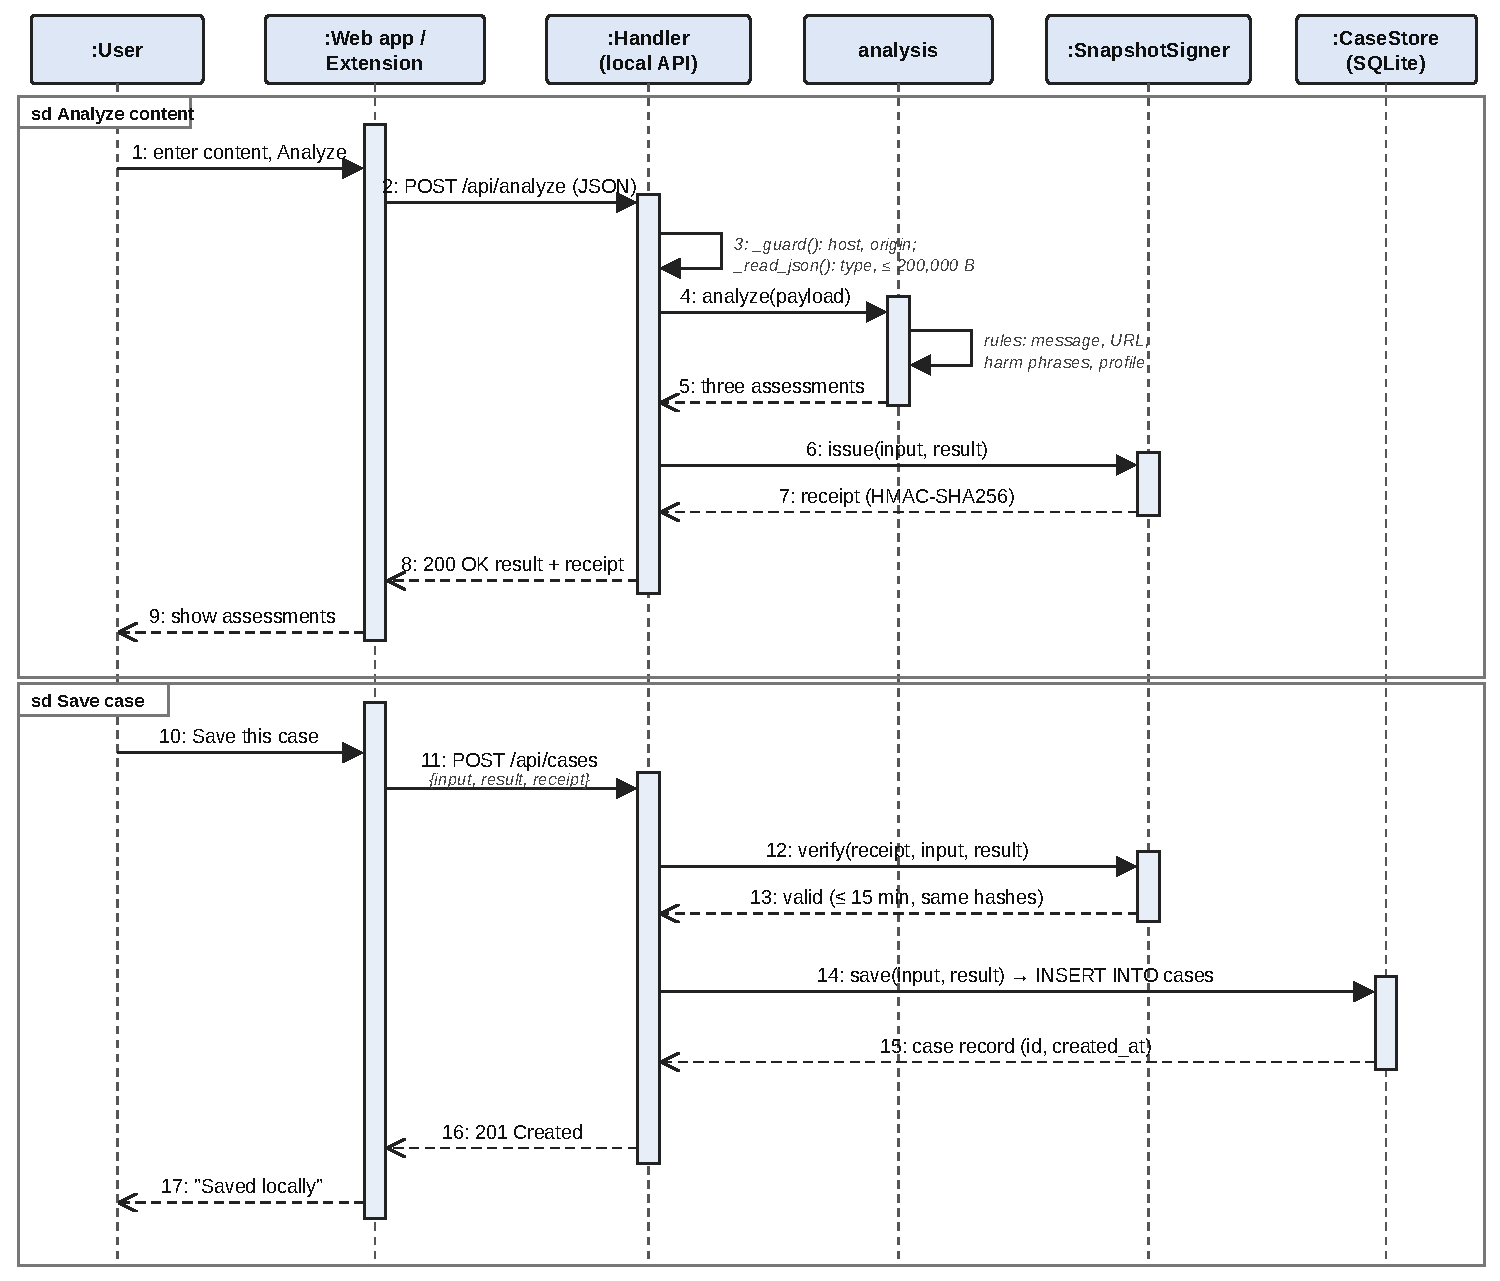
\includegraphics[width=\linewidth]{dia/sequence.pdf}
\caption{Sequence diagram: analysing content and saving a case}
\label{fig:sequence}
\end{figure}
\begin{figure}[H]
\centering
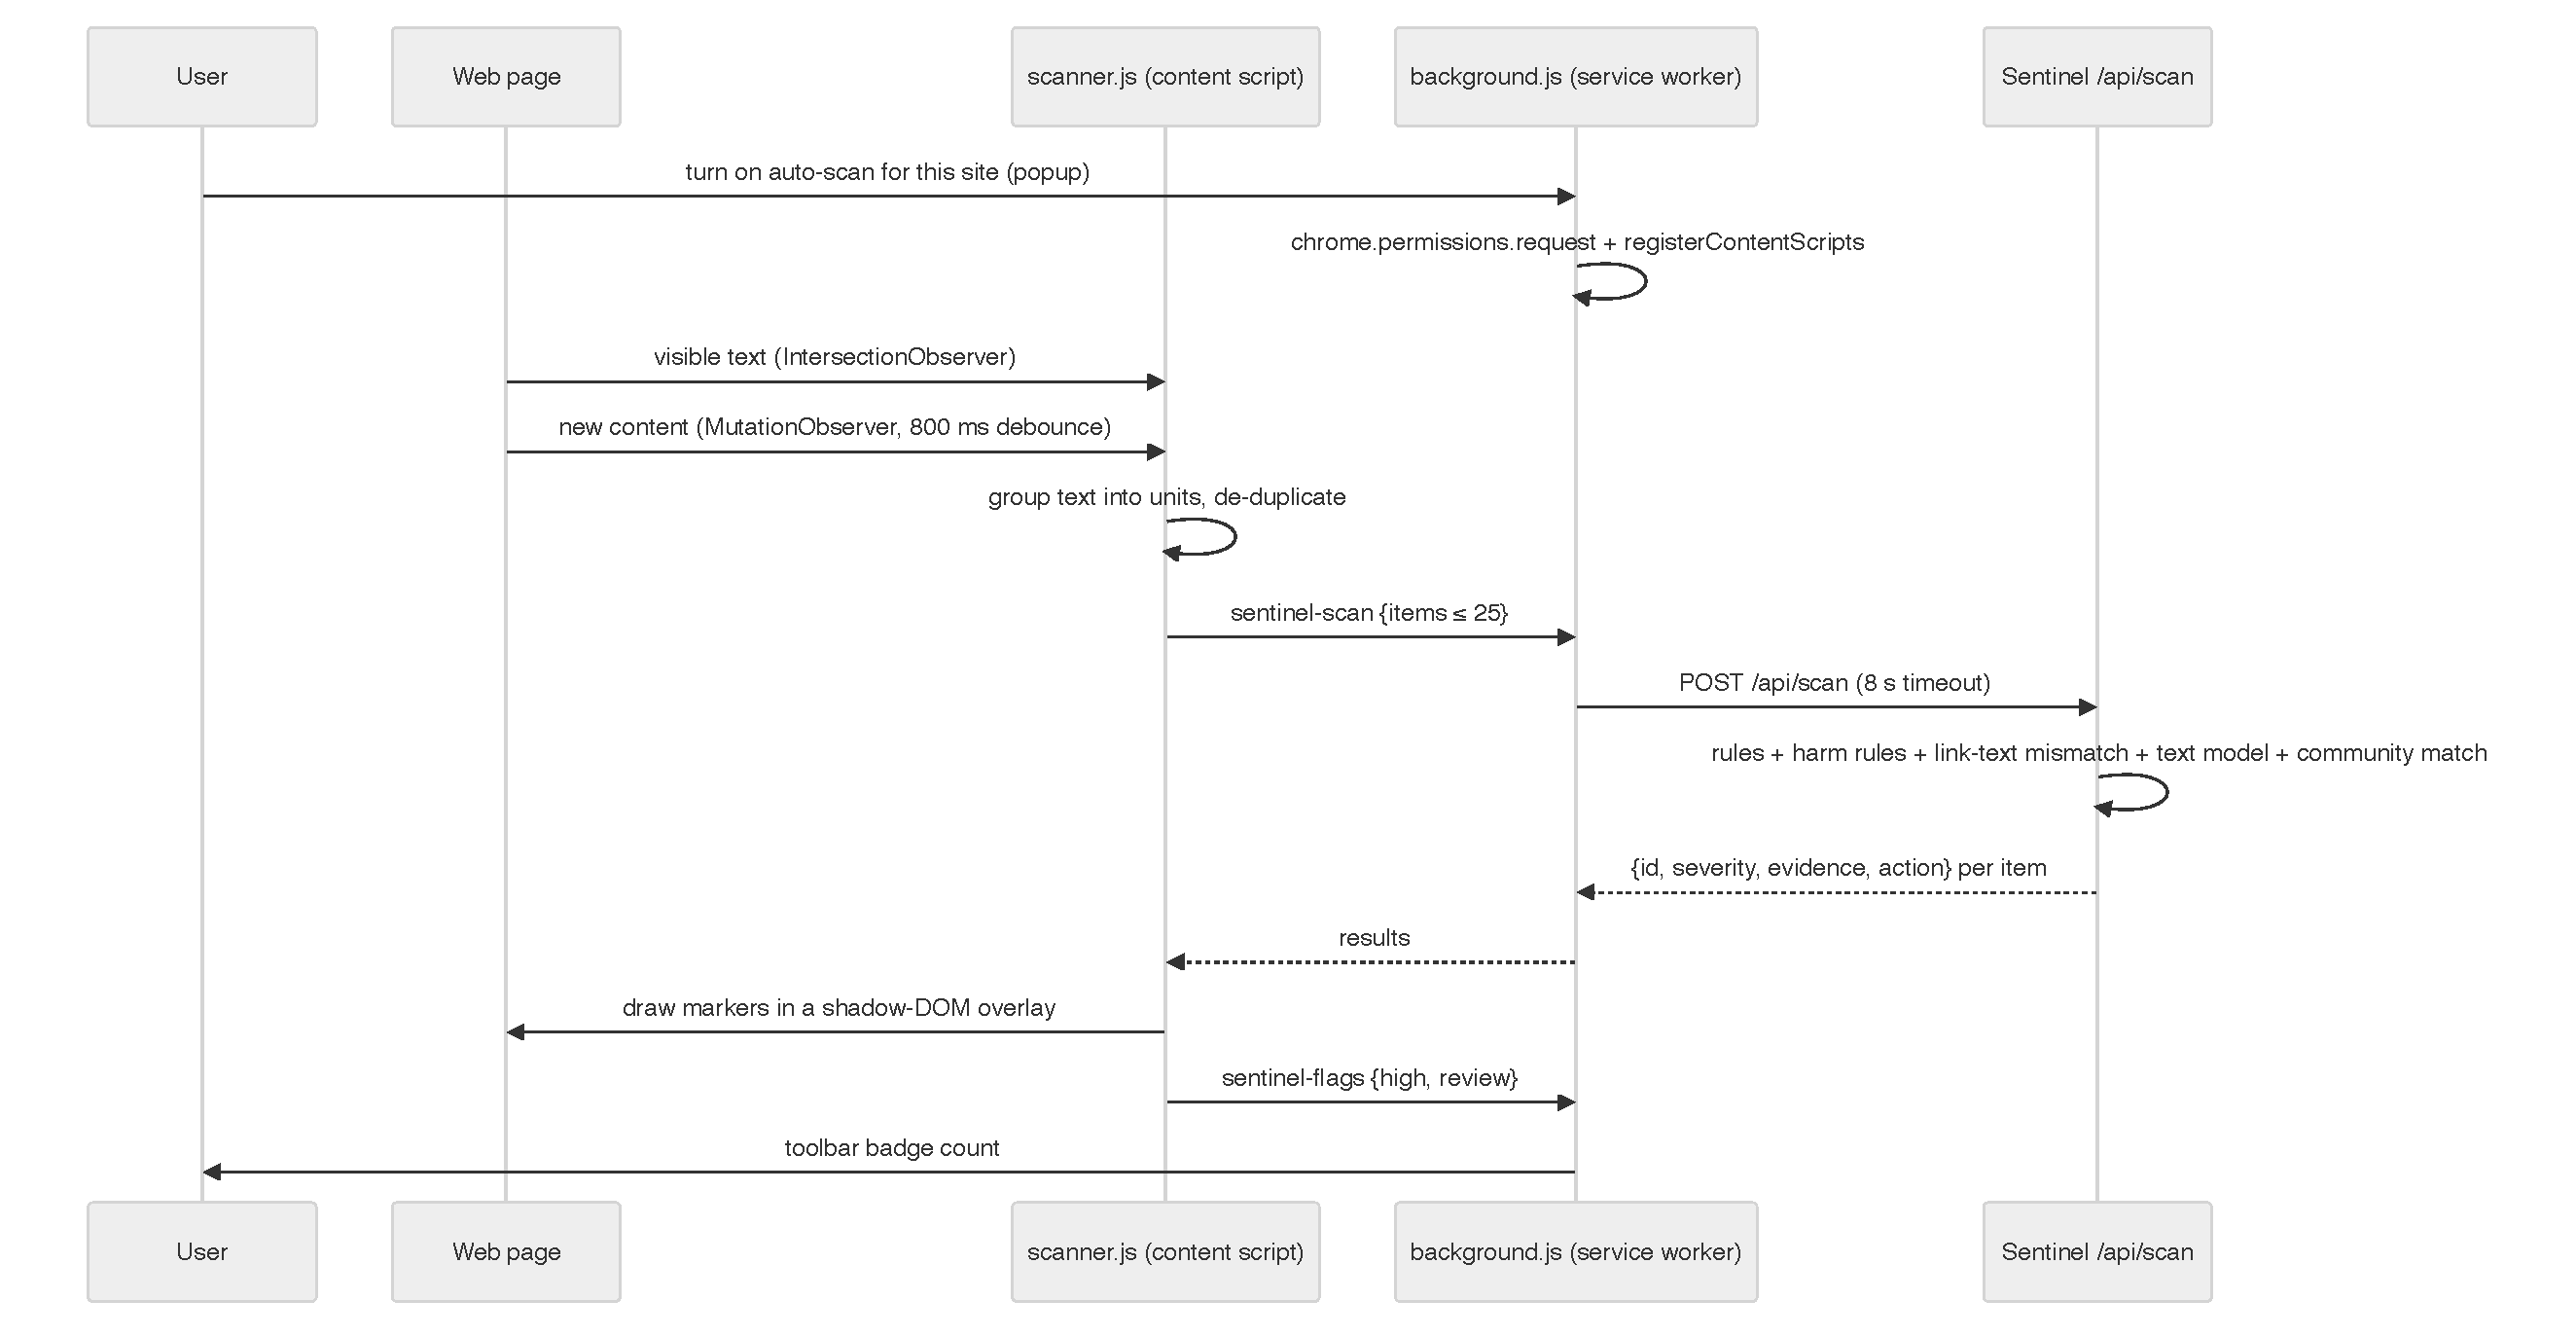
\includegraphics[width=0.92\linewidth]{dia2/autoscan.pdf}
\caption{Sequence diagram: auto-scan of visible page text}
\label{fig:autoscan}
\end{figure}

\subsection{Class Diagram}
\noindent The server creates one case store and one receipt signer, shared by every request handler. The \texttt{analysis} module calls the checkers (Figure~\ref{fig:class}).
\begin{figure}[H]
\centering
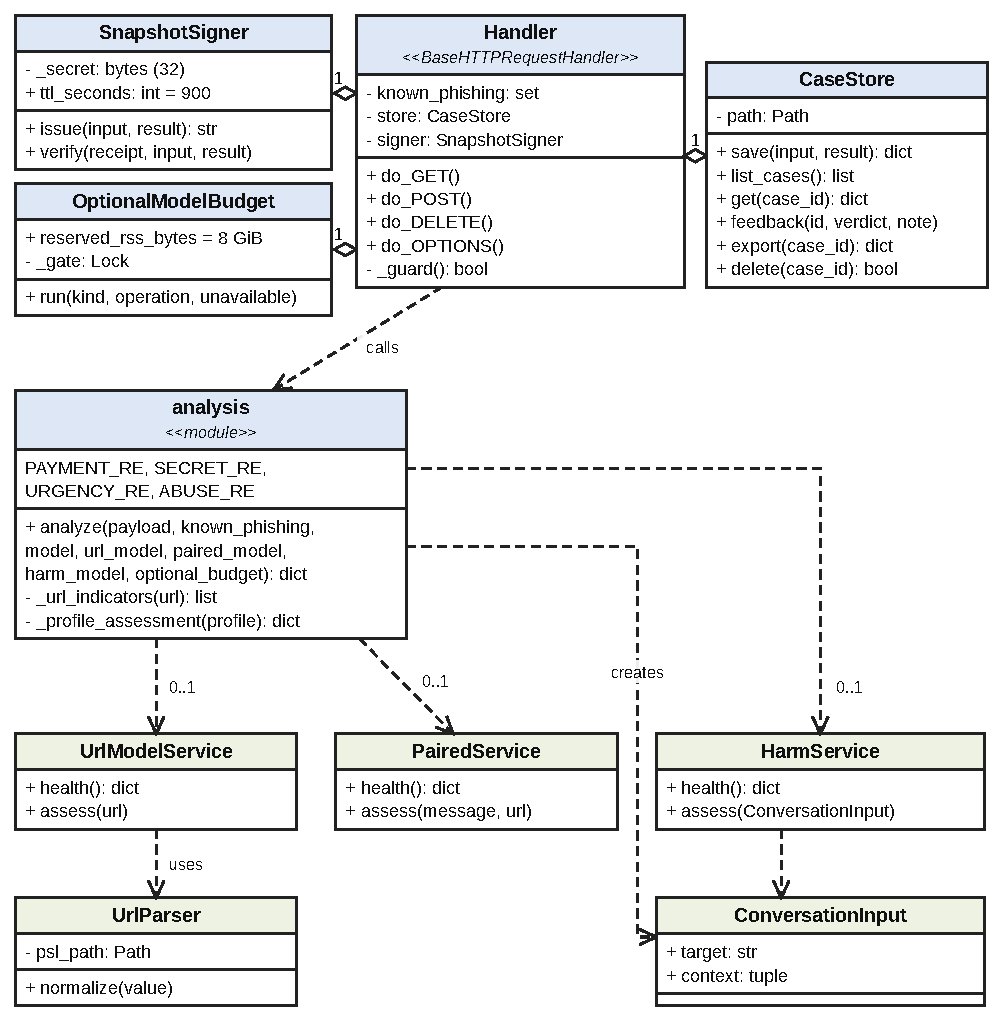
\includegraphics[width=0.78\linewidth]{dia/class.pdf}
\caption{Class diagram of the main application components}
\label{fig:class}
\end{figure}

\subsection{Deployment Diagram}
\noindent Everything runs on the user's computer (Figure~\ref{fig:deploy}): Chrome talks to the Python server, which uses the model files, the case database and, optionally, the community hub and official APIs. Models are trained on a separate research machine and copied over.
\begin{figure}[H]
\centering
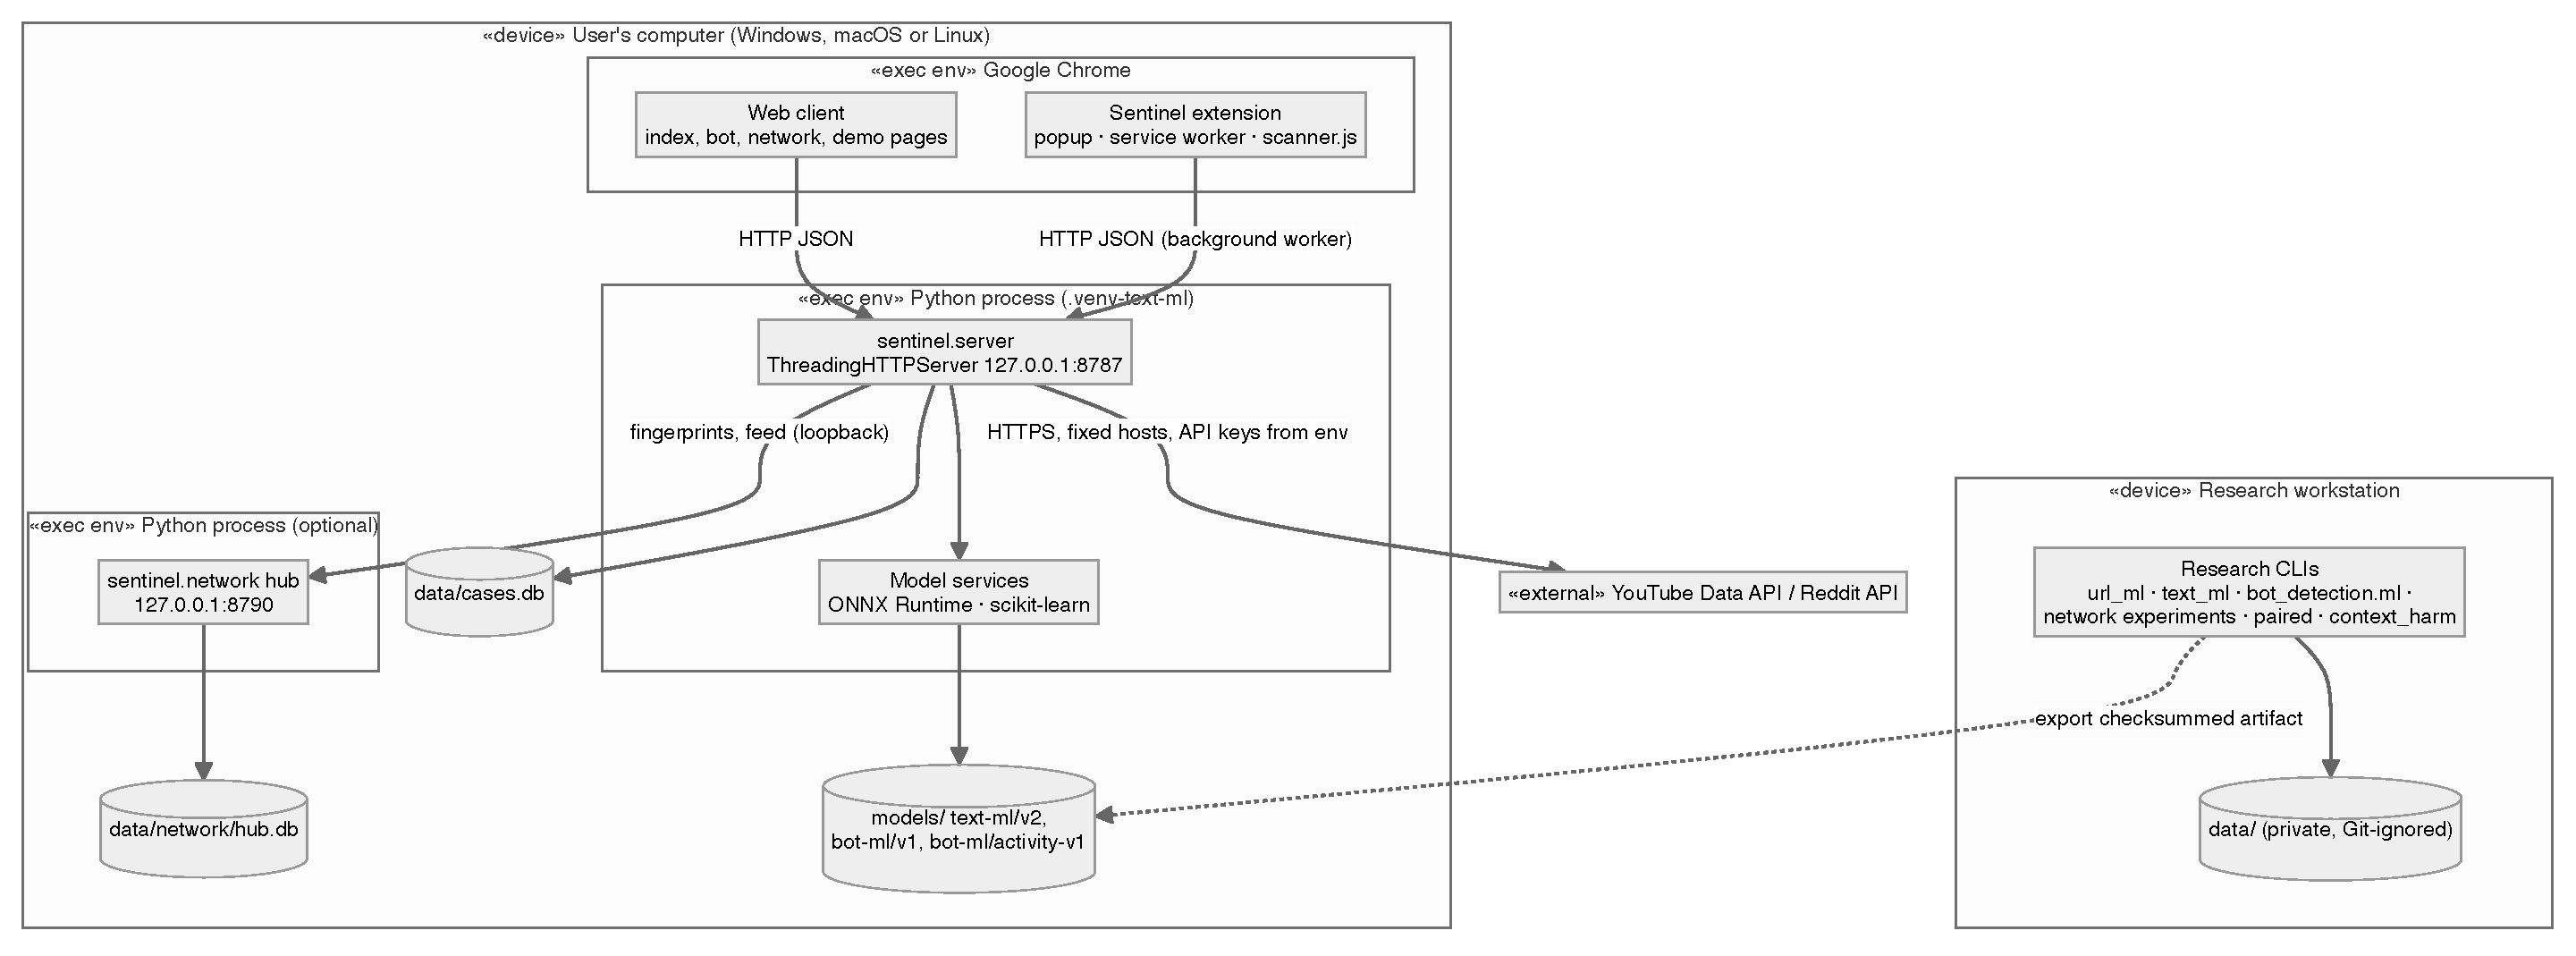
\includegraphics[width=\linewidth]{dia2/deploy_v2.pdf}
\caption{Deployment diagram}
\label{fig:deploy}
\end{figure}

\subsection{ER Diagram and Schema}
\noindent Only saved cases are stored, in one table (Figure~\ref{fig:er}, Table~\ref{tab:schema}). There are no user accounts. The optional hub has its own database of fingerprints, report counts and times, with no message text.
\begin{figure}[H]
\centering
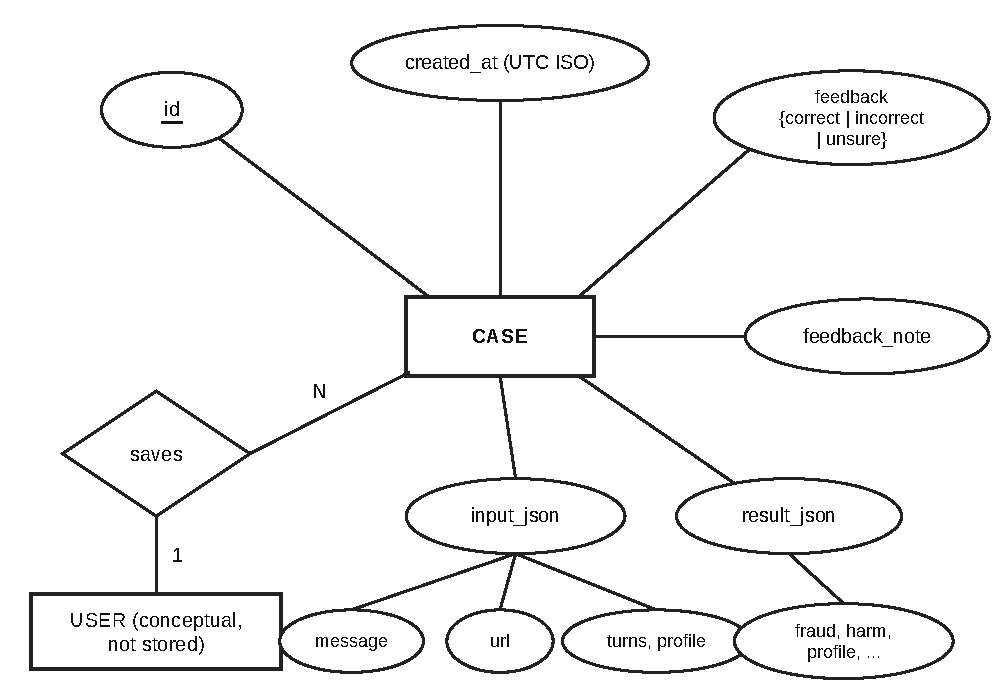
\includegraphics[width=0.62\linewidth]{dia/er.pdf}
\caption{ER diagram of the case store}
\label{fig:er}
\end{figure}
\begin{table}[H]
\centering
\footnotesize
\renewcommand{\arraystretch}{1.15}
\caption{Schema of the \texttt{cases} table}
\label{tab:schema}
\begin{tabular}{|l|l|>{\raggedright\arraybackslash}p{9cm}|}
\hline
\textbf{Column} & \textbf{Type} & \textbf{Meaning} \\ \hline
id & TEXT (key) & Random case ID \\ \hline
created\_at & TEXT & Time saved (UTC) \\ \hline
input\_json & TEXT & What the user checked \\ \hline
result\_json & TEXT & The exact result the user saw \\ \hline
feedback, feedback\_note & TEXT & Optional: correct, incorrect or unsure, with a note \\ \hline
\end{tabular}
\end{table}

\subsection{Data Flow Diagrams}
\noindent At Level 0 (Figure~\ref{fig:dfd0}) Sentinel exchanges content and results with the user, gets known phishing links from a feed and data from public datasets. Level 1 (Figure~\ref{fig:dfd1}) splits it into capturing input, analysing content, managing cases and training models.
\begin{figure}[H]
\centering
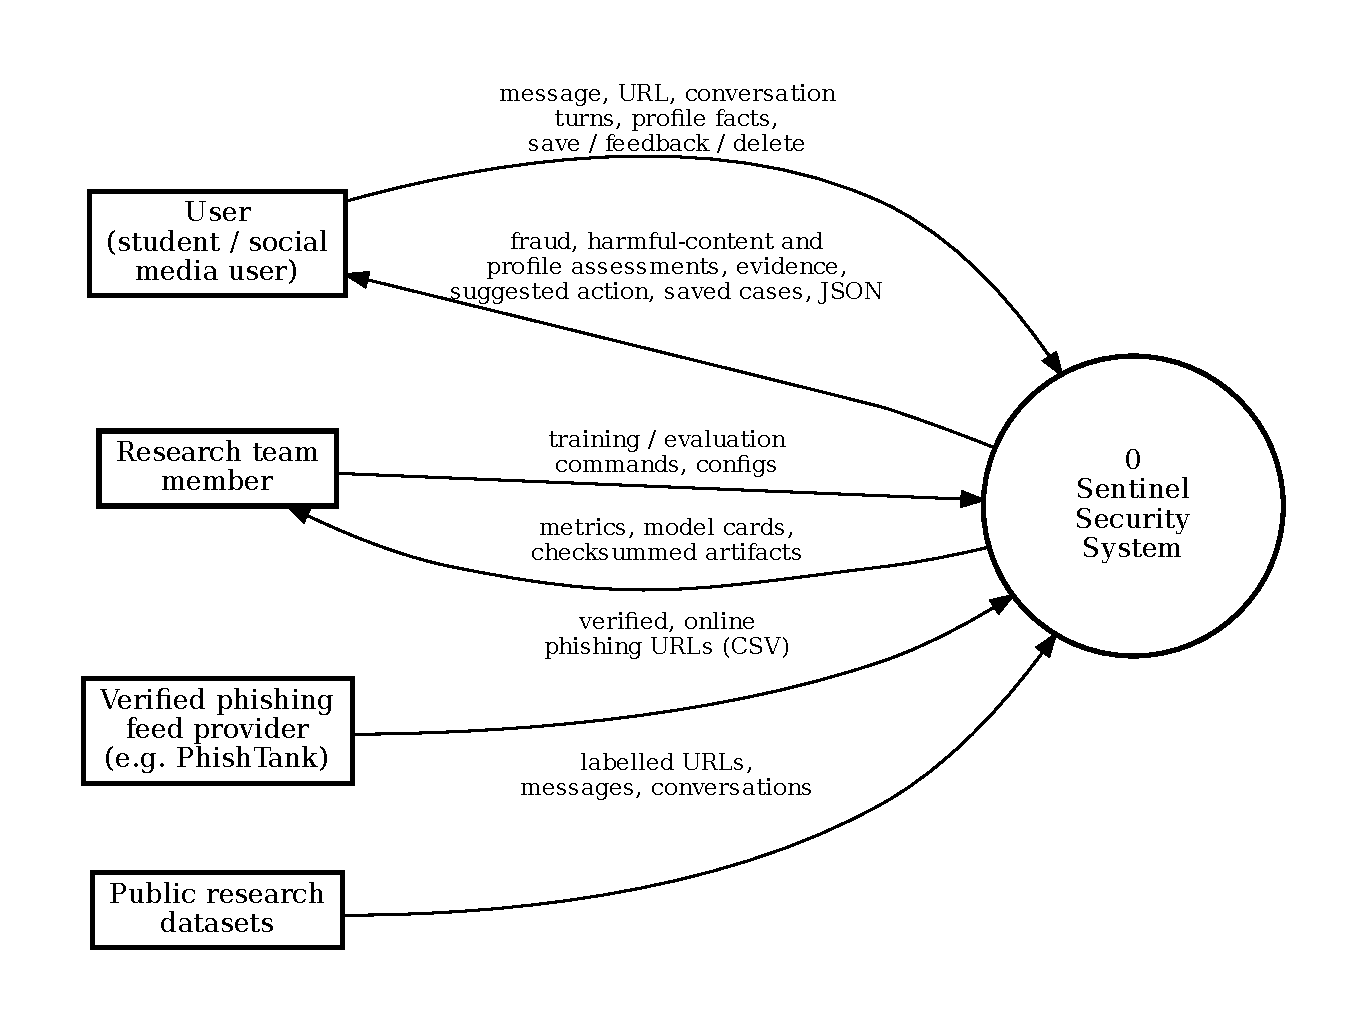
\includegraphics[width=0.72\linewidth]{dia/dfd0.pdf}
\caption{DFD Level 0 (context diagram)}
\label{fig:dfd0}
\end{figure}
\begin{figure}[H]
\centering
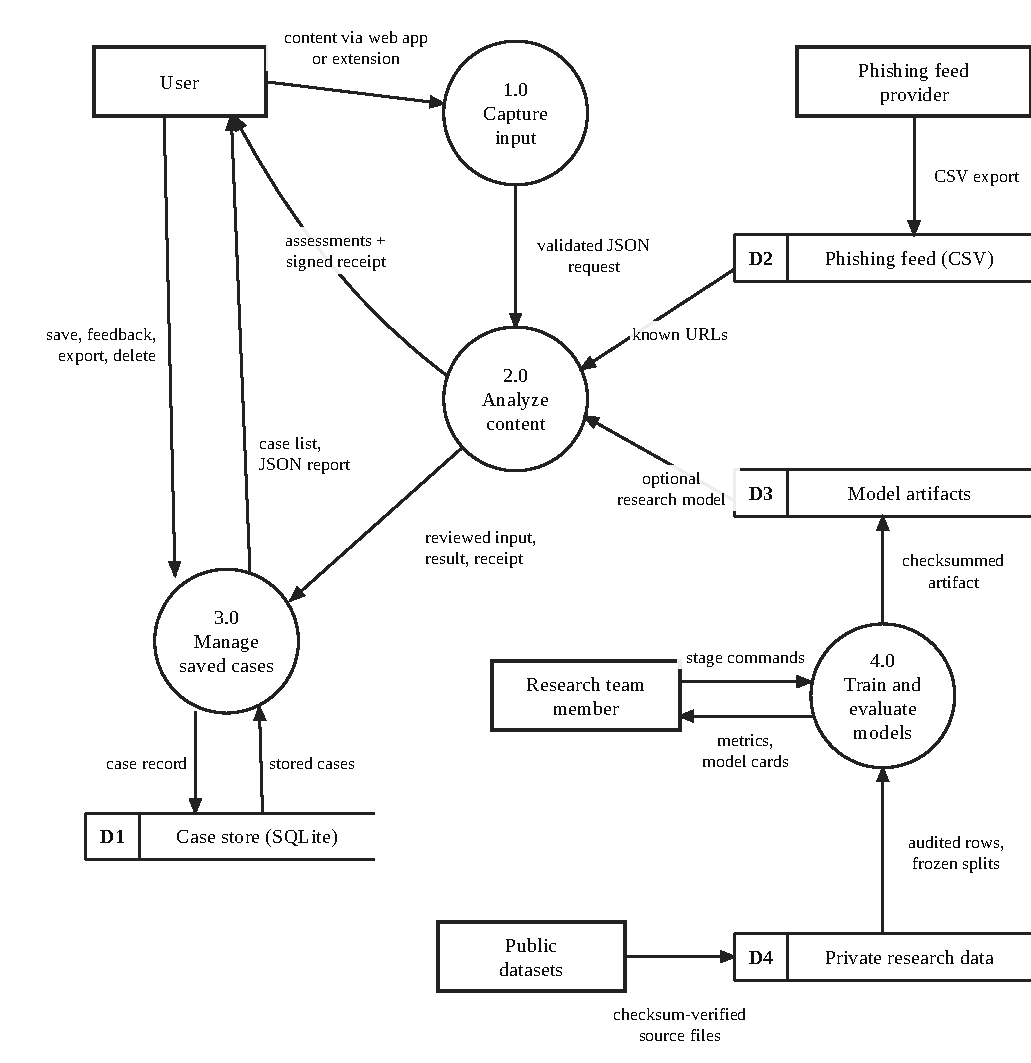
\includegraphics[width=0.78\linewidth]{dia/dfd1.pdf}
\caption{DFD Level 1}
\label{fig:dfd1}
\end{figure}

\subsection{Algorithms and Methodology}\label{sec:algos}
\noindent\textbf{1. Fraud level.} If the link is on the known-phishing list, or the message asks for money or a password \emph{and} the link looks suspicious, the level is \emph{High}. Any other evidence gives \emph{Review}; otherwise \emph{Low observed concern}.\\

\noindent\textbf{2. Harmful language} (Algorithm~\ref{alg:harm}).
\begin{algorithm}[H]
\caption{Harmful-language check}\label{alg:harm}
\begin{algorithmic}[1]
\State clean the text: undo look-alike letters, dotted letters, number-for-letter tricks and stretched letters
\ForAll{each of the 19 rules}
  \State skip matches inside known idioms
  \State if a negation (``never'', ``not'') comes just before: lower the level
  \State if the text is quoted or reported: lower \emph{High} to \emph{Review} (never for self-harm risk)
\EndFor
\State level $\gets$ highest level found; advice $\gets$ advice of the most urgent category
\end{algorithmic}
\end{algorithm}

\noindent\textbf{3. Scam-text model.} DistilBERT's scores are calibrated with a temperature $T=1.29$ and averaged with the TF-IDF model's probabilities $\mathbf{p}^{\mathrm{L}}$:
\begin{equation}
\mathbf{p}=\tfrac12\big(\mathrm{softmax}(\mathbf{z}/T)+\mathbf{p}^{\mathrm{L}}\big),\qquad s=p_{\mathrm{spam}}+p_{\mathrm{smishing}},\qquad \text{warn if } s\ge0.611 .
\end{equation}
The threshold 0.611 was chosen on separate calibration data so that at most 1\% of genuine messages are flagged. To explain a warning, each word is removed in turn and the drop in the score is measured; the biggest drops are shown.\\

\noindent\textbf{4. Community fingerprints.} A message is cut into 3-word pieces, and 64 hash functions give a MinHash fingerprint. Two messages with similarity $J$ share at least one of the 32 fingerprint ``bands'' with probability
\begin{equation}
P(J)=1-\big(1-J^{2}\big)^{32},
\end{equation}
which is 99.7\% at $J=0.41$, so reworded scams still match \cite{mmds}. The hub publishes a scam only after 5 different reporters, gives new users half weight for 24 hours, and removes a campaign if enough users dispute it (Figure~\ref{fig:network}).
\begin{figure}[H]
\centering
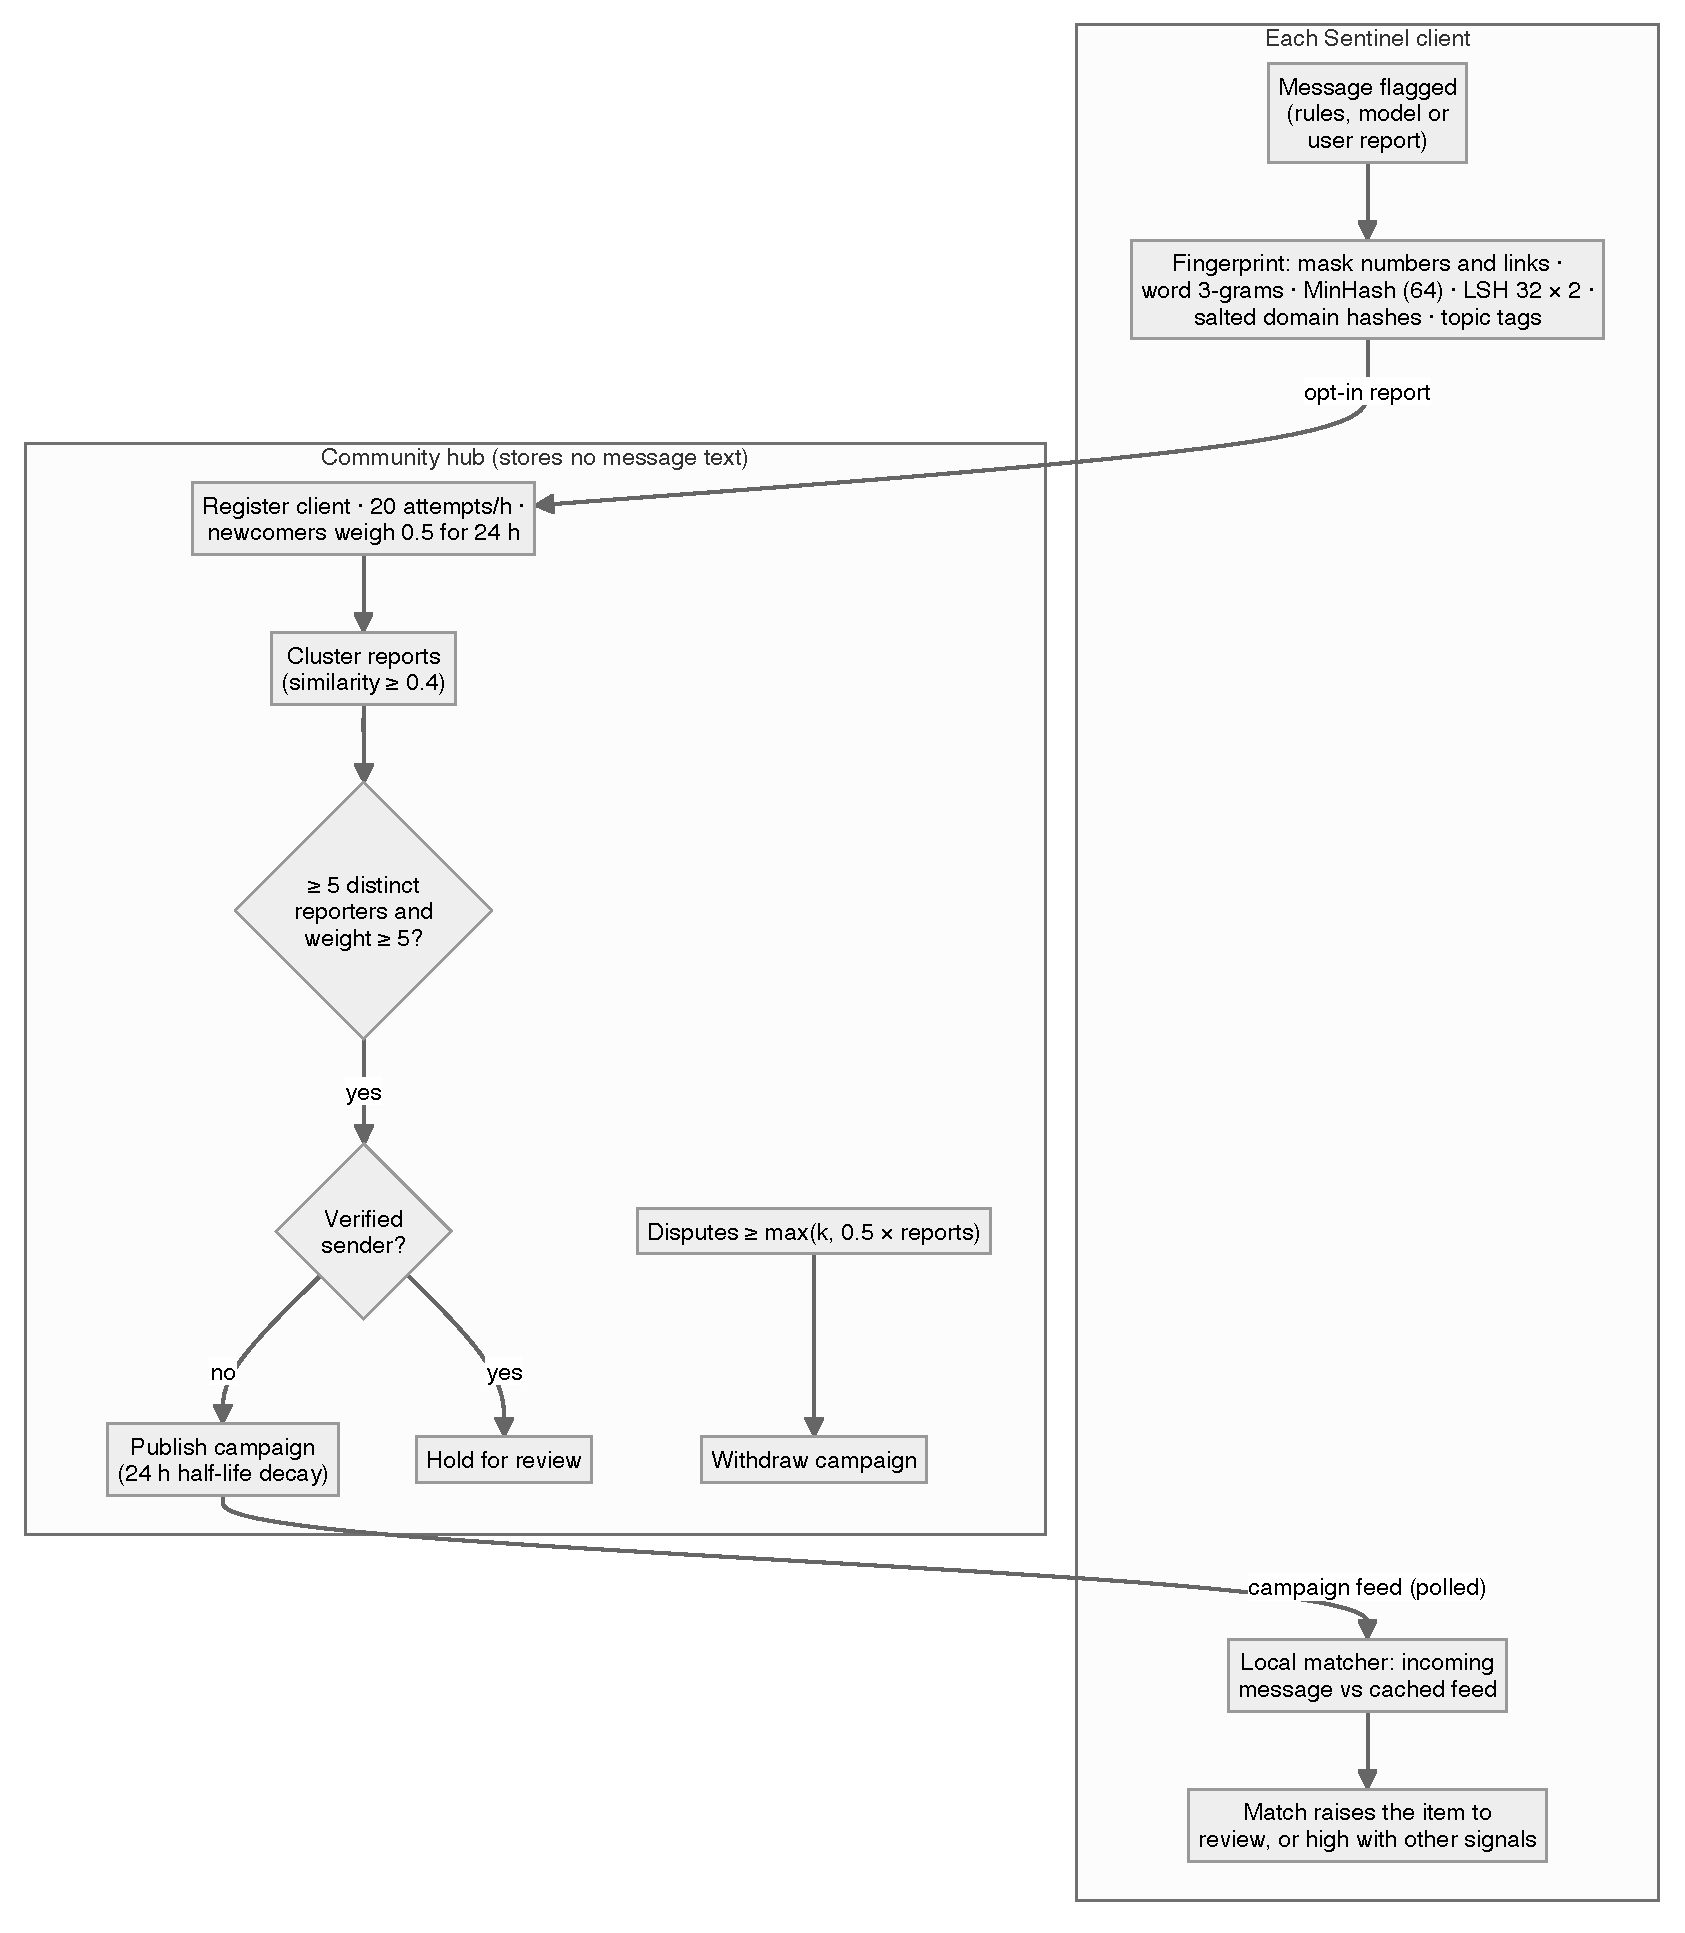
\includegraphics[width=0.55\linewidth]{dia2/network.pdf}
\caption{Community scam network: fingerprinting, publishing and local matching}
\label{fig:network}
\end{figure}

\noindent\textbf{5. Bot score.} Each of the 25 signals gives a suspicion $s_i$ between 0 and 1 and has a weight $w_i$. Only signals with data ($A$) are used:
\begin{equation}
\text{score}=100\cdot\frac{\sum_{i\in A} w_i s_i}{\sum_{i\in A} w_i}.
\end{equation}
If too little data is available (under 25\% of the total weight, or fewer than 4 signals), the score is not shown. For example, bots that post on a timer have almost equal gaps between posts. The trained models use gradient boosting \cite{sklearn} with calibrated probabilities \cite{zadrozny} (Figure~\ref{fig:bot}).
\begin{figure}[H]
\centering
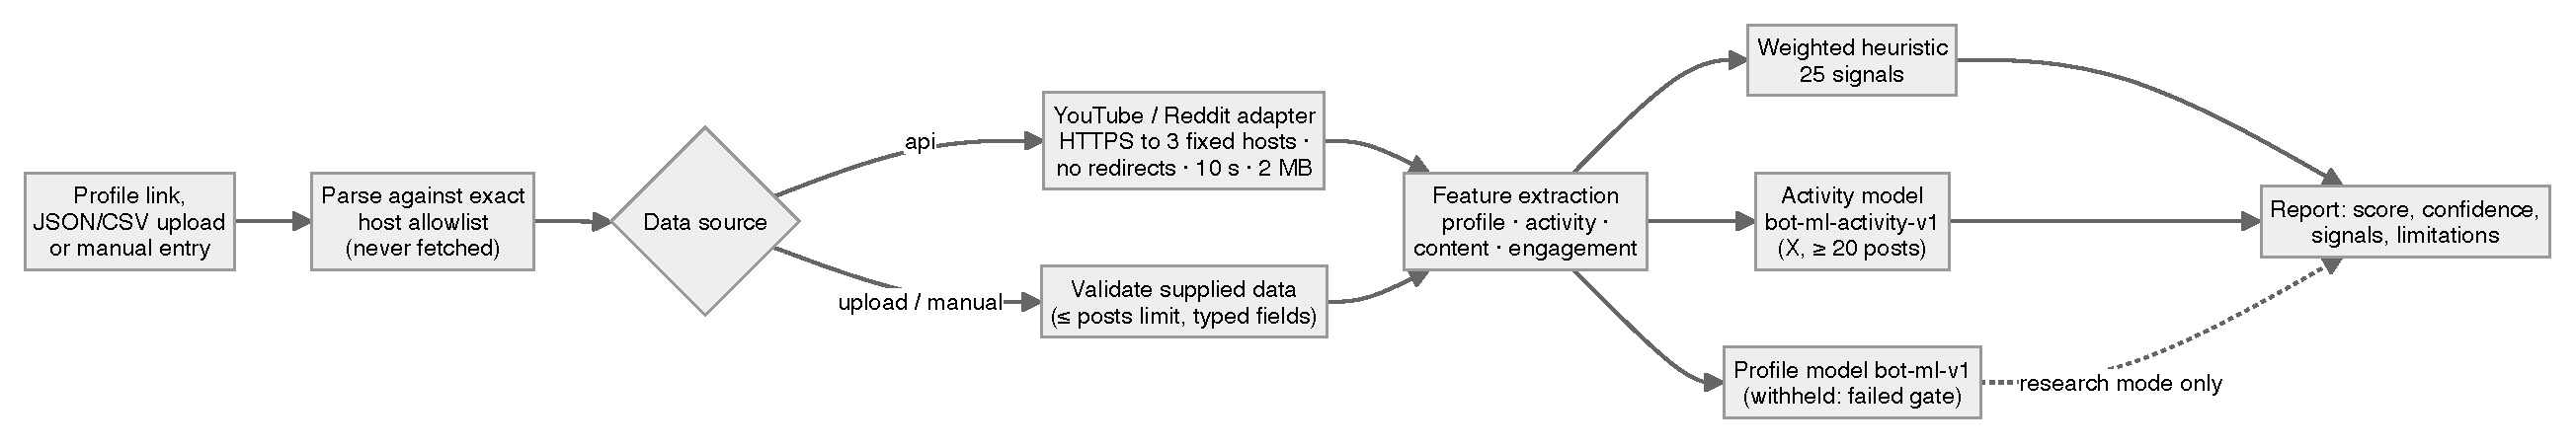
\includegraphics[width=\linewidth]{dia2/bot.pdf}
\caption{Bot-account detection pipeline}
\label{fig:bot}
\end{figure}

\noindent\textbf{6. URL models (research only).} The URL text is split into 3--5 character pieces, turned into TF-IDF features and classified with logistic regression. Data is split by website so that the same site is never in both training and test data.

\subsection{UI/UX Design}
\noindent The design follows four ideas: plain language, separate results for each threat, honesty about limits, and no hidden storage. The check page puts the input on the left and the result cards on the right (Figure~\ref{fig:ui-form}a). Each card shows a level with a text label (not just colour), the evidence, what could not be checked and a next step. The extension popup shows the same cards in a narrow layout (Figure~\ref{fig:ui-form}b; this screenshot is older than the auto-scan switch at the top). The Bot accounts and Community network pages are shown in Figure~\ref{fig:ui-more}.
\begin{figure}[H]
\centering
\begin{minipage}[b]{0.66\linewidth}\centering
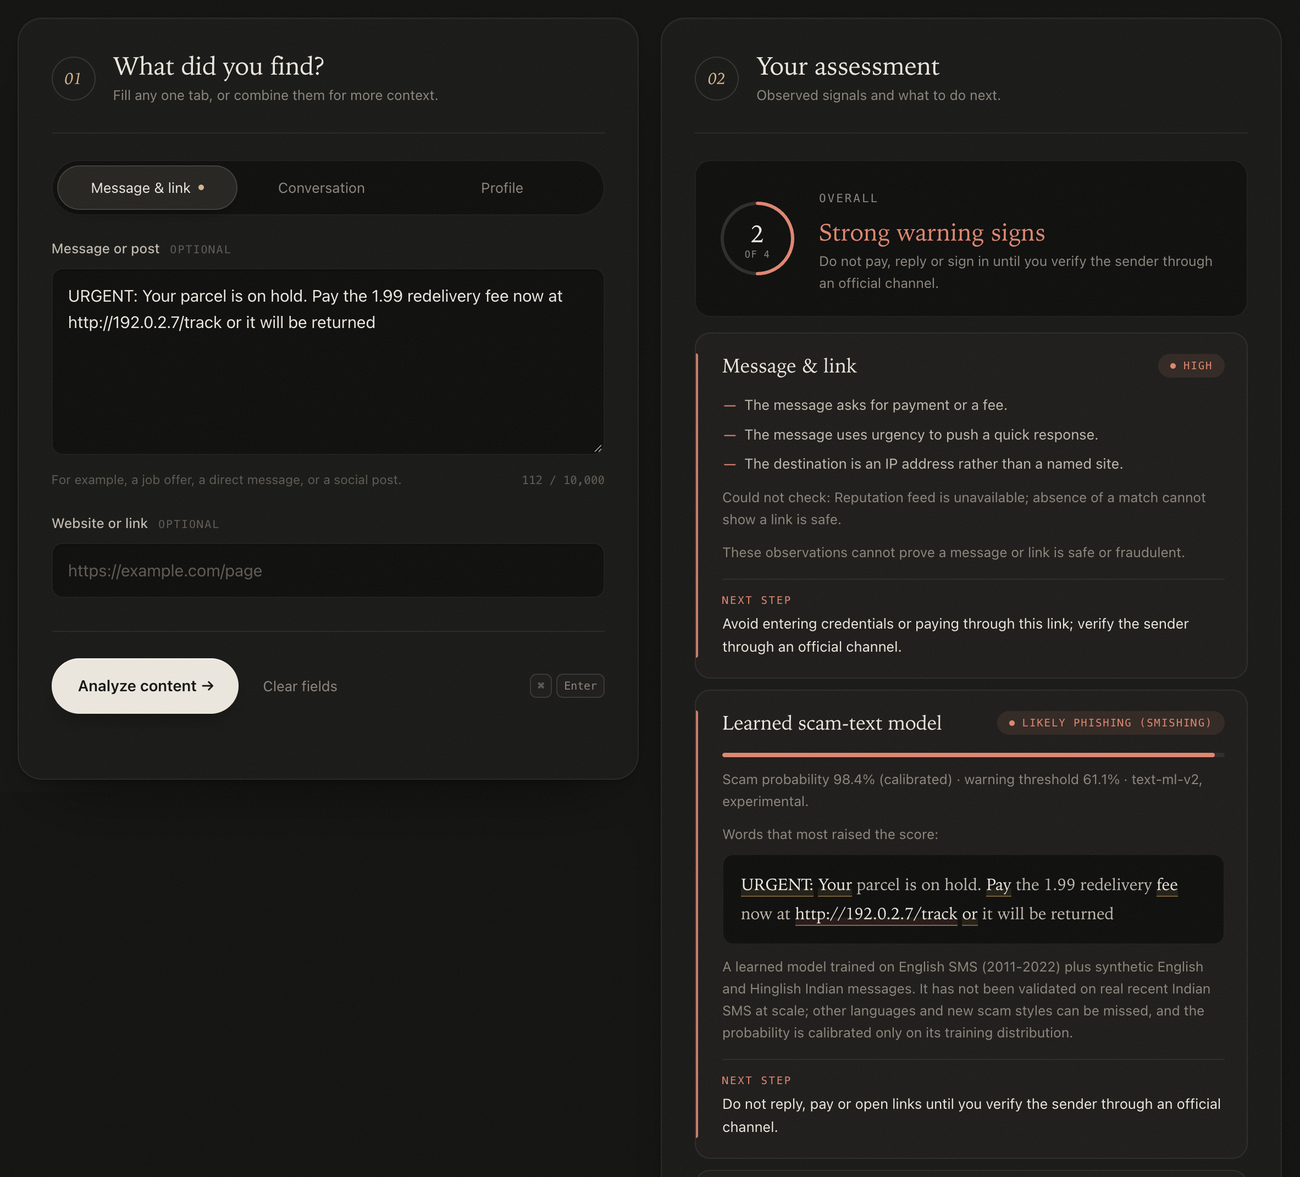
\includegraphics[width=\linewidth]{shots2/check_scam.png}\\[1pt]{\small (a) Check page with a parcel-fee scam}
\end{minipage}\hfill
\begin{minipage}[b]{0.29\linewidth}\centering
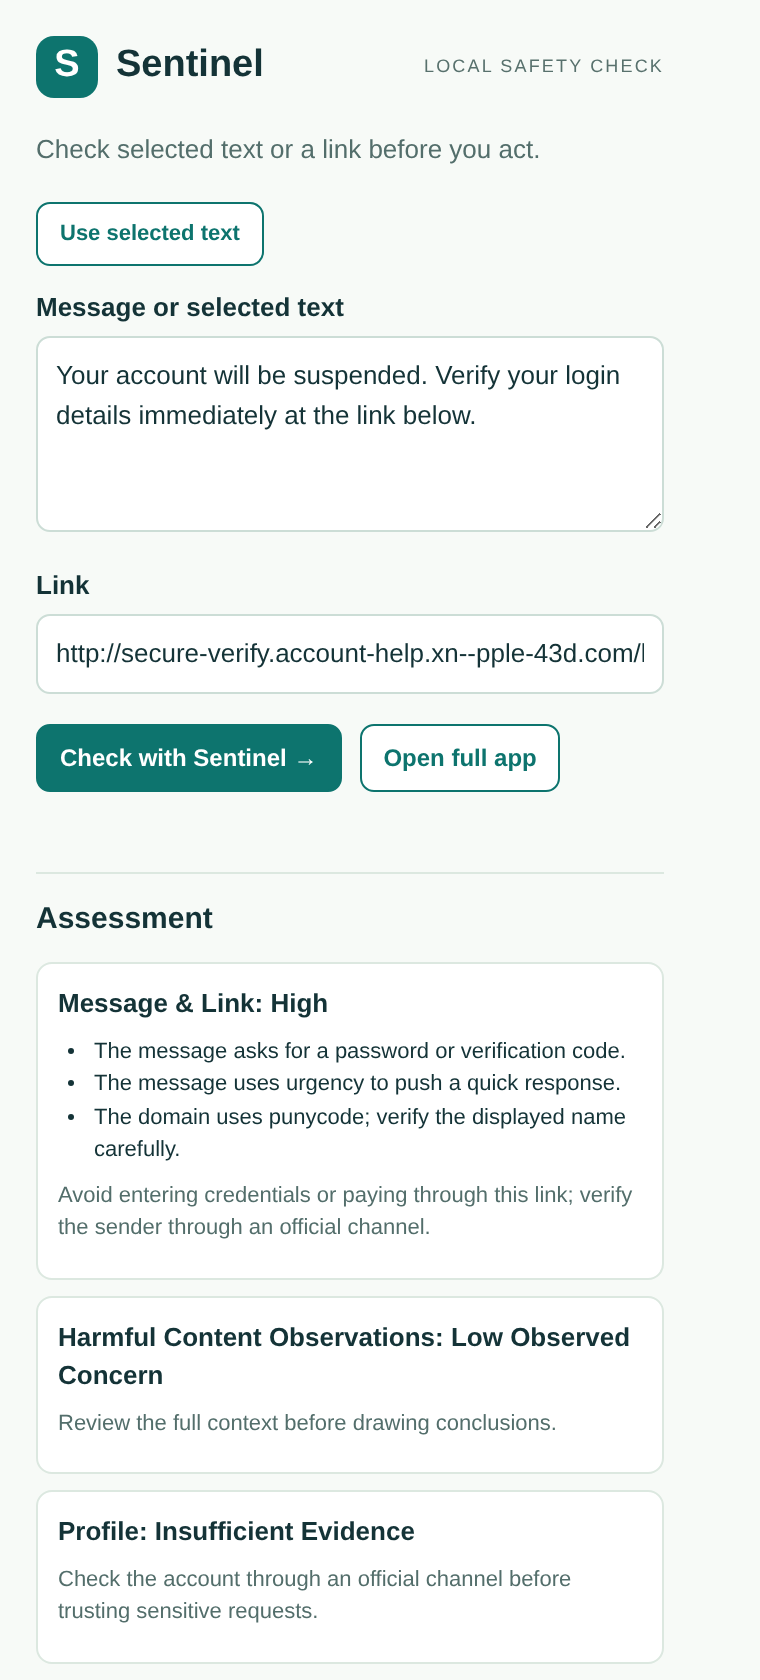
\includegraphics[width=\linewidth]{shots/13_popup_crop.png}\\[1pt]{\small (b) Extension popup}
\end{minipage}
\caption{User interface of Sentinel}
\label{fig:ui-form}
\end{figure}
\begin{figure}[H]
\centering
\begin{minipage}[t]{0.36\linewidth}\centering
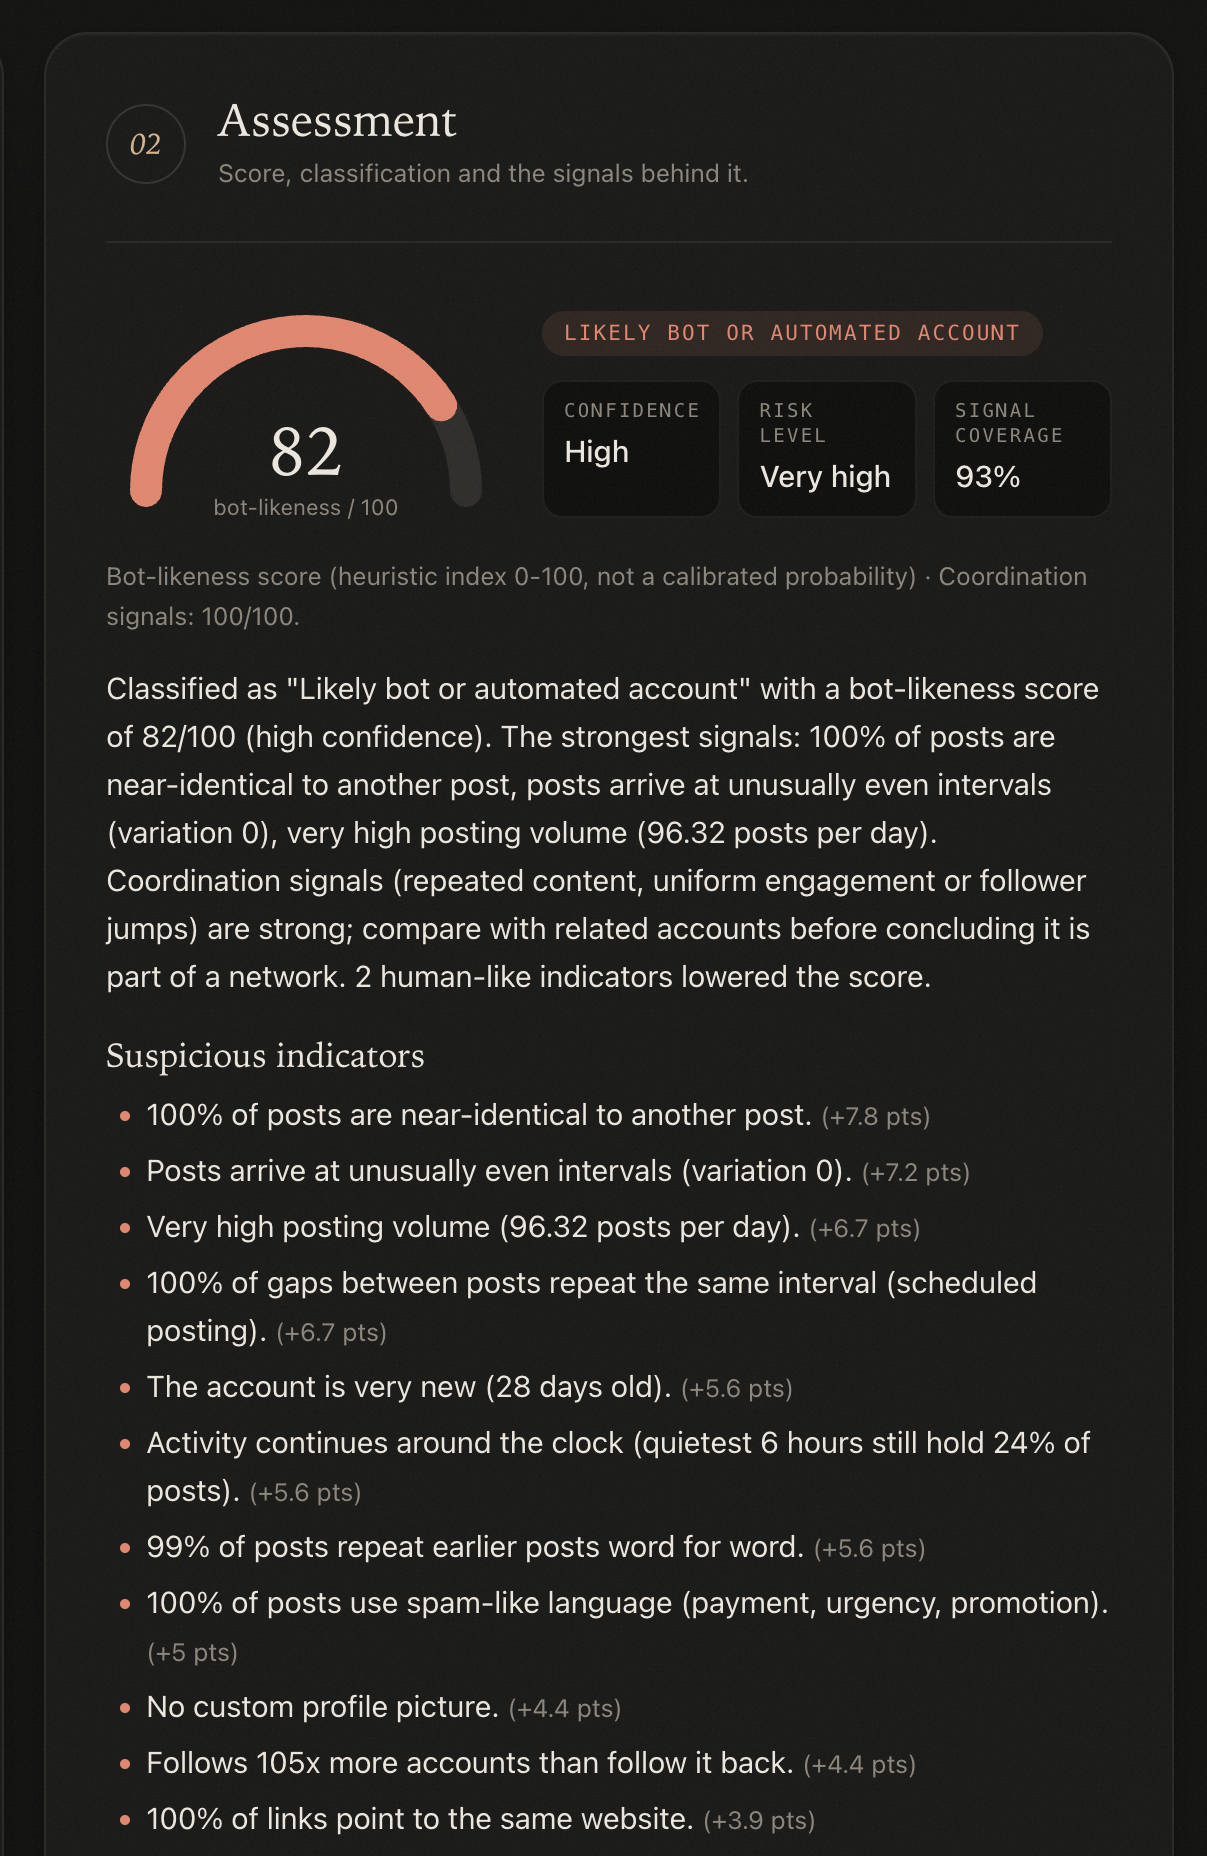
\includegraphics[width=\linewidth]{shots2/bot_report_panel.png}\\[1pt]{\small (a) Bot report for an automated account}
\end{minipage}\hfill
\begin{minipage}[t]{0.6\linewidth}\centering
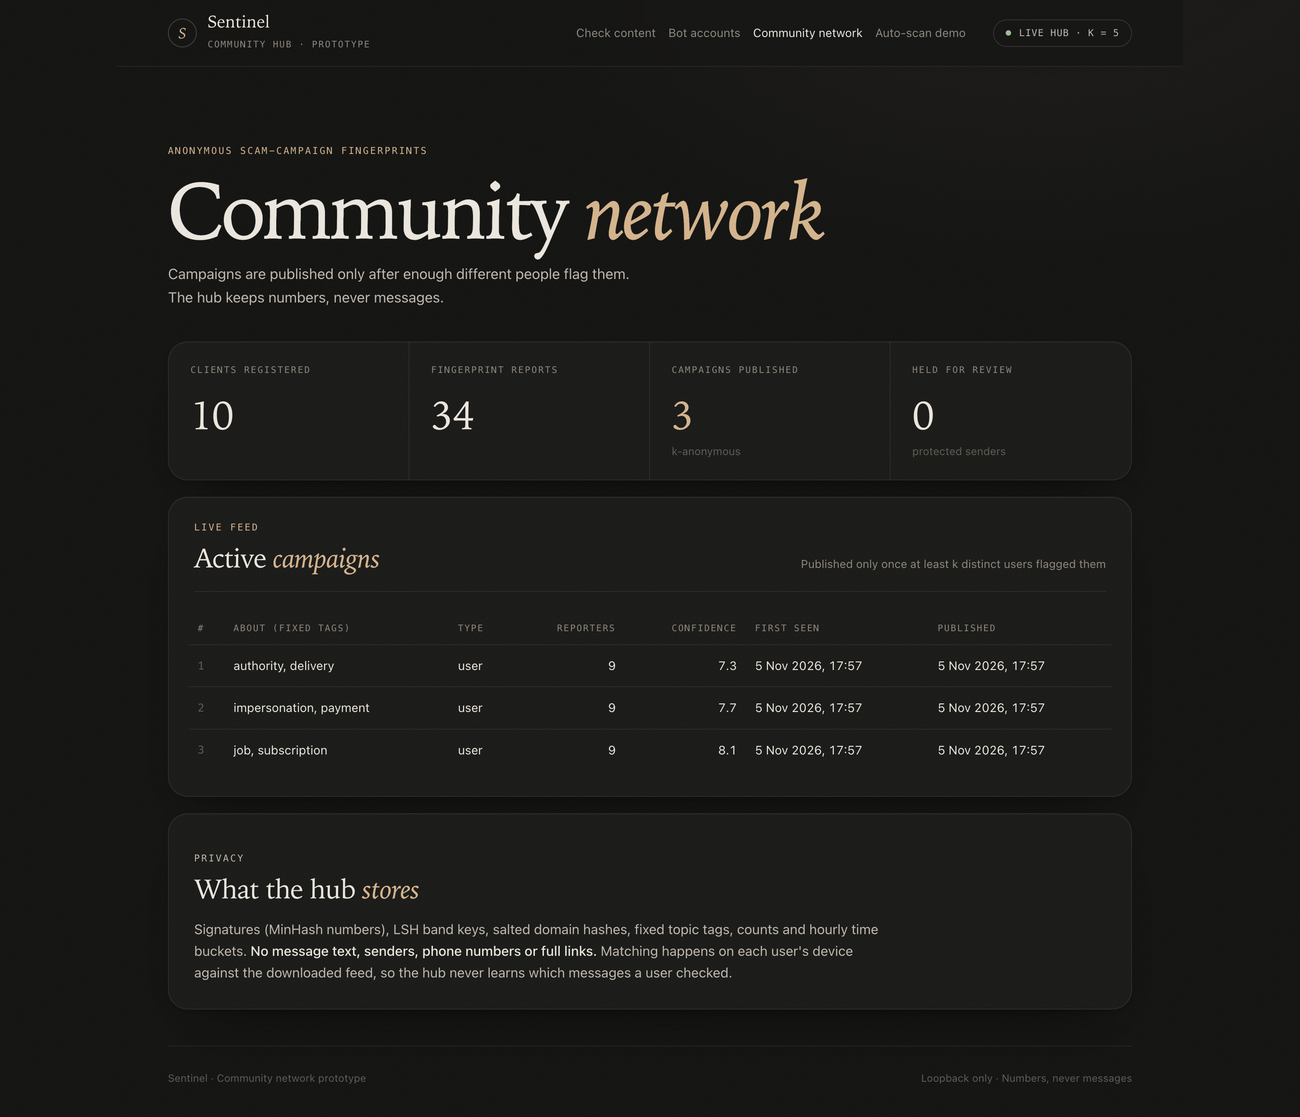
\includegraphics[width=\linewidth]{shots2/network.png}\\[1pt]{\small (b) Community network page}
\end{minipage}
\caption{Bot-detection and community-network pages}
\label{fig:ui-more}
\end{figure}
